\documentclass[a4paper,11pt,french]{article}

%\usepackage[utf8]{inputenc}
%\usepackage[latin1]{inputenc}
%\usepackage[french]{babel}
\usepackage[table]{xcolor}
\usepackage{fancyhdr}
\usepackage{tabularx}
\usepackage{longtable}
\usepackage[pdftex]{graphicx}  


\usepackage[utf8x]{inputenc}
\usepackage[francais]{babel}
\usepackage[T1]{fontenc}

\begin{document}

\title{Le manuel de GuiPG}
\author{Pierre \bsc{Balmelle}, Lucas \bsc{Barbay}, Bertille \bsc{Bouillie}, Mathieu \bsc{Fin}, \\ Guillaume \bsc{Leroy}, Ibrahima \bsc{Sory Barry}, Olivier \bsc{Thibault}}
\maketitle

\normalsize
\clearpage
\tableofcontents
\clearpage

\section{Introduction}

GuiPG est une interface graphique basique pour GnuPG, un outil de chiffrement. GnuPG (aussi connu sous le nom de gpg) est inclus dans la plupart des distributions et est probablement installé sur votre système. Vous pouvez obtenir la dernière version sur http ://gnupg.org.
Avec GuiPG, vous pourrez chiffrer et déchiffrer vos fichiers ou vos courriers électroniques, permettant ainsi des communications plus sécurisées. Un petit guide sur le chiffrement avec gpg est disponible sur le site de GnuPG.
Avec GuiPG, vous n’avez pas besoin de connaître les lignes de commandes et les options du programme gpg. Tout ou presque peut être réalisé par le biais de l'interface.

\section{Présentation de l'interface}

Voici l'interface de GuiPG : \bigbreak

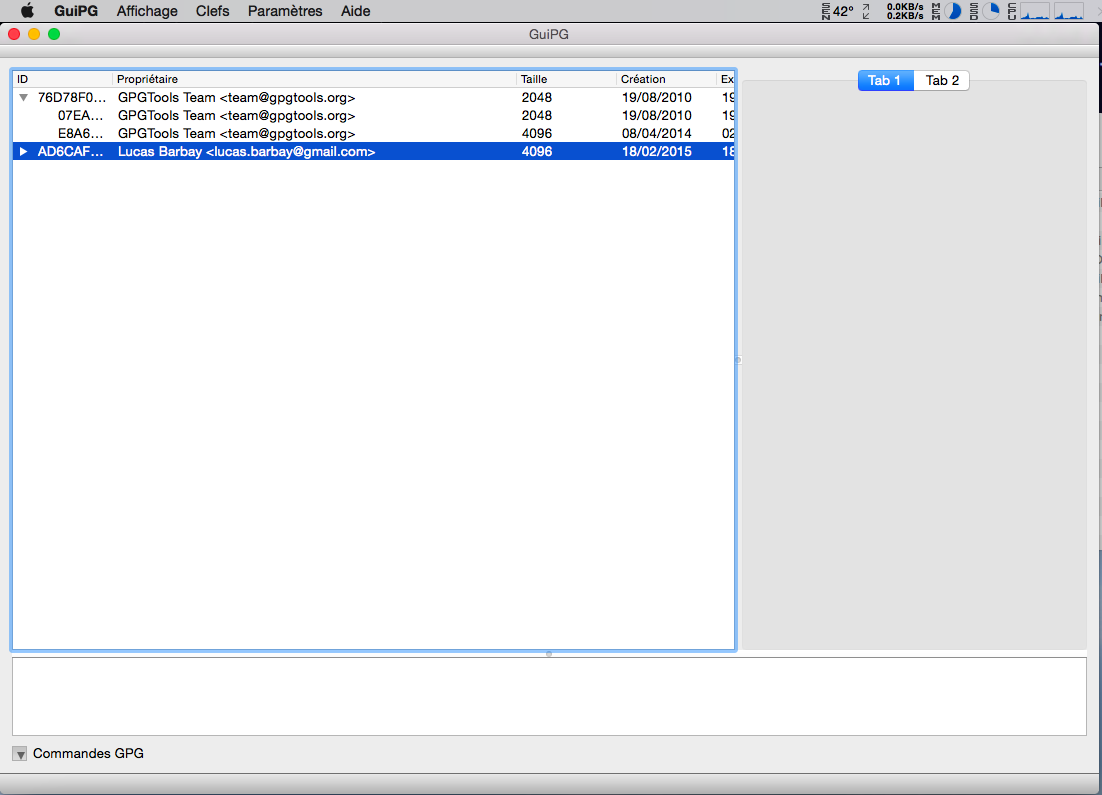
\includegraphics[scale=0.3]{interface.png} \bigbreak

Vous pouvez voir que cette interface est divisée en trois : 
\begin{itemize}
\item Une partie à gauche qui nous permettra de lister les clefs de notre trousseau ainsi que ses sous-clefs. Cette liste est représentée sous forme d'arbre pour mieux visualiser les sous-clefs.
\item Une partie droite contenant deux onglets.
\item Une partie console en bas qui listera les commandes à chaque fois qu'une action GnuPG sera lancée par le biais de l'interface
\end{itemize}

\section{Utilisation de GuiPG}

\subsection{Gestion des profils}

Vous pouvez utiliser plusieurs profils dans GuiPG. Chaque profil est constitué d'un nom, d'un chemin vers GPG ainsi que de la version utilisée. Cela permet d'utiliser différentes versions de GPG (1.4 ou 2) compatibles avec GuiPG. La fenêtre de gestion de profil est la suivante et permet la création, suppression ou le chargement d'un
profil. \bigbreak

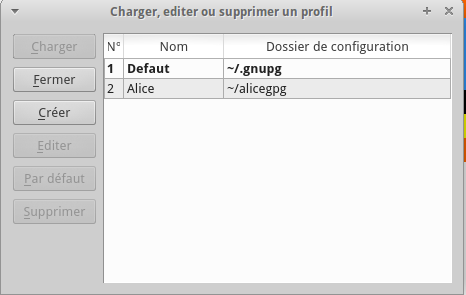
\includegraphics[scale=0.5]{profil.png}


\subsection{Création d'une clef GPG}


La fenêtre permettant de générer une clef est accessible depuis l'onglet Clefs puis Générer une paire de clefs. \bigbreak

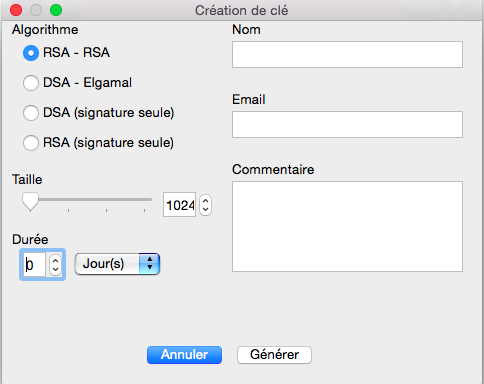
\includegraphics[scale=0.5]{creation.png} \bigbreak


Dans cette fenêtre, il faut remplir les différentes champs qui vont constituer la clef (le nom, l'adresse mail et optionnellement un commentaire). 
Vous avez le choix de garder les paramètres de génération par défaut ou bien vous pouvez par exemple choisir l'algorithme de chiffrement, la taille de la clef ou encore
la durée de votre clef. Si vous avez peur de perdre votre mot de passe, il est conseillé de mettre une durée d'un an de la clef pour éviter qu'elle reste valable. Il est
ensuite possible de changer la durée de vie de cette clef si vous souhaitez la conserver plus longtemps.

\section{Remerciements et licence}

Nous remercions Magalie BARDET qui nous a permis de développer cette interface dans le cadre de notre Master 1 SSI. GuiPG est la propriété de l'Université de Rouen.




\end{document}